\subsection{O(n)}
The computational expense of evaluating the fitness of a TM will vary depending on the particular implementation of the fitness algorithm. The use of an interpreted programming language also provides a challenge with regard to computational expense. For this research it was necessary to evaluate the computational expense for this particular fitness algorithm and implementation in ruby. 

For each of the three fitness evaluation algorithms the computational expense of a single fitness evaluation was less than .2 seconds. At this level of computational expense it was not necessary to consider parallel execution implementations for the GA. However, if other fitness algorithms were used which increased the computational cost of a single evaluation to approximately 1 second or longer it would be beneficial to consider parallel computing. To help keep the computational cost down, the length of the output tape for each TM was limited to a maximum length of 5000 bits. When the tape reaches that length the TM is forced to halt. This restriction is somewhat artificial, but it helps to keep the computational cost down. It also prevents TM with very long, but very simple outputs from scoring much higher than more random but shorter outputs. By setting the maximum length 

GAs lend themselves to parallel computation because for a given population, each member of the population can be evaluated independently of all the other. This allows GAs to be constructed using Message Passing Interface (MPI) which can make use of multiprocessor machines and network based computational clusters. 

\subsection{Optimization Results}
Each of the three types of fitness algorithms were tested by running three separate optimizations. All of the optimizations were run with the same control parameters: 
\begin{itemize}
\item NUM\_STATES: 64
\item GENE\_LENGTH: 2
\item population size: 100
\item generations: 100
\end{itemize}
The generational history for each optimization is presented in Figure \ref{fig:results_metrics}. The maximum fitness overall was 55. The initial average fitness of the first generation was nearly 0, but the initial maximum fitness was 48. The difference of only 7 points between the initial and the final maximum fitness indicates that there was not a significant increase in output complexity discovered over the course of the optimization. The deflate compression algorithm used to compress the output strings displays a small preference for heavily repeating patterns, and it is possible that this small difference reflects this tendency. However, it is also possible that these optimization results represent the maximum complexity achievable in a 5000 bit output tape. 


\begin{figure}[!htb]
  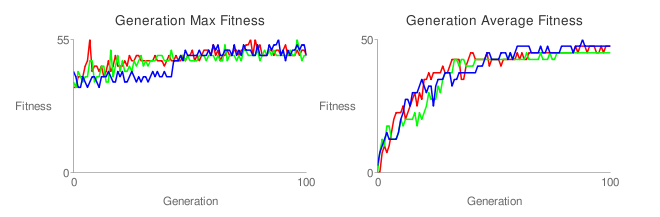
\includegraphics[width=.85\textwidth]{images/results_metrics.png}
  \caption{Final optimization results for three optimizations. Red: random input tape, Green: constant input tape, Blue: Slow drift input tape \label{fig:results_metrics}}
\end{figure}

When comparing the results between each of the three separate fitness evaluation techniques, from Figure \ref{fig:results_metrics} it is obvious that none of the three methods hold a significant advantage in finding a more complex machine. In all three cases, by the 50th generation the optimization rate slowed to a low enough speed that further optimization was not necessary. In fact, in the case of the random input tape case, the red line, the overall maximum fitness was actually discovered very early on and rediscovered much later on. 

One stated goal of the optimization was to maintain as much population diversity as possible. The average fitness data history provides an indication of the relative diversity and how it changed over course of the optimization. As the generations progressed the average fitness starts out near zero. It climbs very quickly as the weakest of the population die out first. The average fitness begins to approach the maximum fitness as the generations progress because the population begins to converge on the strongest candidates. Once the population reaches a certain amount of homogeneity the optimization it is unlikely that any new members will emerge with a strong advantage over the others because the gene pool is too small. At this point, only mutation could provide the necessary injection of new genetic material. Because of the large potential non-coding regions of the 64 state encodings, it is possible that a mutation would turn on a dormant part of the genome and allow for a strong advantage, but in this optimization all three methods had approximately 50 generations to allow this to happen and it did not. 

Since none of the three variations in fitness algorithms produced significantly improved results, it is fair to conclude that none of them provides a significantly different result than any of the others. It is interesting that all three input methods result in similar TM whose output reaches a similar amount of complexity. 

One notable aspect of the results is the oscillating results. This effect is most notable in the red data, the random input tape method. This optimization reached a maximum early on and took a few generations to refind a TM with similarly complex output. This effect is notable because it illuminated a potential weakness in the GA used. This GA does not ensure that the strongest population member of a generation survives to the next generation. It is highly likely that it will survive, but in the event that a single population candidate becomes significantly stronger in a single generation, it is possible despite its overwhelming strength it will not survive to the next generation. If it does not survive, its genetic material is lost and would need to be rediscovered later. This property is mostly a consequence of the selection method used, competition with only two contestants. This method was used to help ensure maximum diversity, but it also has the side effect of increasing the probability that a single strong population member would not get to enter a competition and so it would never win one and never reproduce. This problem could be remedied by either increasing the size of competitions or by switching to a roulette selection method. Either solution would greatly increase the chance that the best candidate will survive. 

Neither of these methods will absolutely guarantee that the strongest candidates survive. It is, of course, possible to simply always pass the strongest population member to the next generation. However, doing so moves the algorithm away from mimicking nature as closely as possible. In nature, there is no guarantee that even very strong organism will have a chance to mate. Any number of things can happen to prevent it to happen, like a pretator or some natural distator. Future research could investigate the efficacy of trying to always preserve the strongest candidates, either by increasing their chance of survival or by simply making it happen. 